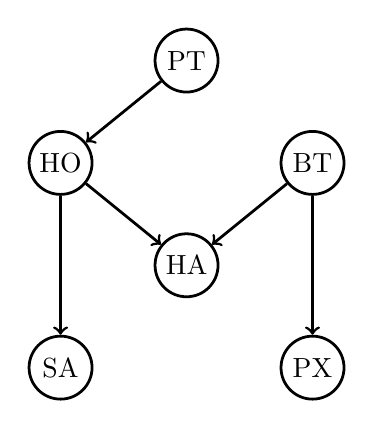
\begin{tikzpicture}[line width = 1pt,
                    x = 1.6cm,
                    y = 1.3cm,
                    node/.style = {circle, draw, inner sep = 0pt, minimum size = 0.8cm}]

    % \grid{0}{15}{0}{13}
    \node[node] (PT) at (1,3) {PT};
    \node[node] (HO) at (0,2) {HO};
    \node[node] (BT) at (2,2) {BT};
    \node[node] (SA) at (0,0) {SA};
    \node[node] (PX) at (2,0) {PX};
    \node[node] (HA) at (1,1) {HA};

    \foreach \i/\j in {PT/HO,
                       HO/HA,
                       BT/HA,
                       HO/SA,
                       BT/PX}
    {
        \draw[->] (\i) -- (\j);
    }
\end{tikzpicture}